\subsection{Casi di studio}
\begin{figure}[thp]
\centering
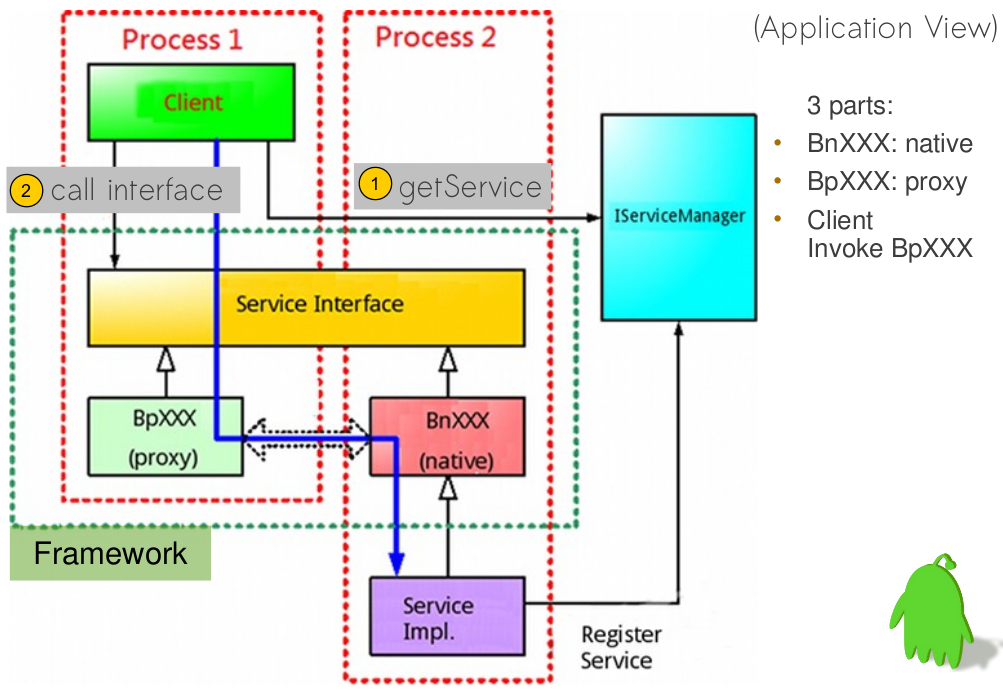
\includegraphics[scale=0.43]{img/korea/cpplevel.png}
\caption{\textit{Gerarchia delle classi lato applicazioni in codice nativo C++. \parencite{slide:zhIPC}}.}
\label{subfig:zhcpplevel}
\end{figure}

\textit{All'interno di questa sottosezione, mostrerò i principali meccanismi di
registrazione ed ottenimento di servizi, sia lato nativo, sia lato Java, allo 
scopo di tralasciare questi dettagli nella descrizione delle interazioni
osservate in Sezione \vref{sec:rivsupuser}. Discorrerò quindi di:}
\begin{itemize}
\diam Registrazione di \textit{service} nativi: v. \vref{subsub:regservicenative}.
\diam Invocazione di RPC da codice nativo: v. \vref{subsub:evokrpcfromnative}.
\diam Registrazione dei servizi lato Java: v. \vref{subsec:regserv}.
\diam Invocazione di metodi Java da Native Code: v. \vref{subsec:invoke}.
\end{itemize}

Per una prima visione d'insieme, mostro la Figura \vref{subfig:zhcpplevel}: 
come si può notare, il codice C++
fornisce l'implementazione per interagire con i metodi definiti da un'interfaccia
\texttt{\small IXXX}: vengono allo scopo definiti le classi \texttt{\small BpXXX} e 
\texttt{\small BnXXX}, del quale il Listato \vref{alg:ipcontrol} fornisce un esempio.
Come possiamo notare, il programma cliente interagirà con l'oggetto del tipo
\texttt{\small BpXXX} il quale, grazie al Binder, riuscirà ad interagire con un 
altro oggetto \texttt{\small BnXXX}, esteso da un servizio che lo implementa: questo
è necessario in quanto questa classe non implementa tutti i 
metodi necessari all'effettiva esecuzione del codice che sono lasciati \texttt{\small virtual},
come il metodo \texttt{\small checkPermission} in esso definito. 

\begin{algorithm}[thp]
\begin{cpp}[caption=$ $IPermissionController.cpp,label=alg:ipcontrol]
namespace android {

// ----------------------------------------------------------------------

class BpPermissionController : public BpInterface<IPermissionController>
{
public:
    BpPermissionController(const sp<IBinder>& impl)
        : BpInterface<IPermissionController>(impl)
    {
    }

    virtual bool checkPermission(const String16& permission, int32_t pid, int32_t uid)
    {
        Parcel data, reply;
        data.writeInterfaceToken(IPermissionController::getInterfaceDescriptor());
        data.writeString16(permission);
        data.writeInt32(pid);
        data.writeInt32(uid);
        remote()->transact(CHECK_PERMISSION_TRANSACTION, data, &reply);
        // fail on exception
        if (reply.readExceptionCode() != 0) return 0;
        return reply.readInt32() != 0;
    }
};

IMPLEMENT_META_INTERFACE(PermissionController, "android.os.IPermissionController");

// ----------------------------------------------------------------------

status_t BnPermissionController::onTransact(
    uint32_t code, const Parcel& data, Parcel* reply, uint32_t flags)
{
    //printf("PermissionController received: "); data.print();
    switch(code) {
        case CHECK_PERMISSION_TRANSACTION: {
            CHECK_INTERFACE(IPermissionController, data, reply);
            String16 permission = data.readString16();
            int32_t pid = data.readInt32();
            int32_t uid = data.readInt32();
            bool res = checkPermission(permission, pid, uid);
            reply->writeNoException();
            reply->writeInt32(res ? 1 : 0);
            return NO_ERROR;
        } break;
        default:
            return BBinder::onTransact(code, data, reply, flags);
    }
}

}
\end{cpp}
\end{algorithm}



\subsubsection{Registrazione di \textit{service} nativi}\label{subsub:regservicenative}
Prima di poter effettuare la registrazione di un \textit{service} nativo, è 
opportuno ottenere un \textit{proxy} per la comunicazione con il \textit{Service Manager}:
questo è ottenibile tramite il metodo \texttt{\small defaultServiceManager} il quale,
o richiama un'istanza \textit{singleton} precedentemente creata per tutto il sistema,
oppure ricorre a crearne una nuova tramite il metodo \texttt{\small getContextObject(caller)}
tramite \texttt{\small ProcessState}.

Come osservabile dal Listato che segue, si utilizza un
particolare oggetto, detto \texttt{\small ProcessState}, per mettersi in 
comunicazione con il Binder, ed in particolare per aprire il suddetto device
\footnote{In particolare all'interno dell'ultimo sorgente AOSP si riscontrano
 delle differenze di implementazione da quelle evidenziate in \parencite{site:anonBinder}.}
\begin{cpp}[caption=$ $IServiceManager.cpp]
sp<IServiceManager> defaultServiceManager()
{
    if (gDefaultServiceManager != NULL) return gDefaultServiceManager;
    
    {
        AutoMutex _l(gDefaultServiceManagerLock);
        if (gDefaultServiceManager == NULL) {
            gDefaultServiceManager = interface_cast<IServiceManager>(
                ProcessState::self()->getContextObject(NULL));
        }
    }
    
    return gDefaultServiceManager;
}
\end{cpp}

In particolare il costruttore di tale oggetto viene definito nel seguente modo:
\begin{cpp}[caption=$ $(1) ProcessState.cpp ]
ProcessState::ProcessState()
    : mDriverFD(open_driver())
    , mVMStart(MAP_FAILED)
    , mManagesContexts(false)
    , mBinderContextCheckFunc(NULL)
    , mBinderContextUserData(NULL)
    , mThreadPoolStarted(false)
    , mThreadPoolSeq(1)
{
    if (mDriverFD >= 0) {
        // XXX Ideally, there should be a specific define for whether we
        // have mmap (or whether we could possibly have the kernel module
        // availabla).
#if !defined(HAVE_WIN32_IPC)
        // mmap the binder, providing a chunk of virtual address space to receive transactions.
        mVMStart = mmap(0, BINDER_VM_SIZE, PROT_READ, MAP_PRIVATE | MAP_NORESERVE, mDriverFD, 0);
        if (mVMStart == MAP_FAILED) {
            // *sigh*
            ALOGE("Using /dev/binder failed: unable to mmap transaction memory.\n");
            close(mDriverFD);
            mDriverFD = -1;
        }
#else
        mDriverFD = -1;
#endif
    }

    LOG_ALWAYS_FATAL_IF(mDriverFD < 0, "Binder driver could not be opened.  Terminating.");
}
\end{cpp}
Si riscontra come si apra il device in questione e si effettui il \textit{mapping}
di una regione di memoria, allo scopo di ricevere le transazioni: quest'ultima
utility è in particolare utilizzata dai \textit{service}
per ricevere le richieste dai client. In particolare dal metodo \texttt{\small getContextObject}
viene sempre restituito un oggetto di tipo \texttt{\small BpBinder} il quale,
conoscendo lo \textit{hanlde} associato, ovvero il numero assegnato dal Binder
al servizio richiesto, che nel caso del \textit{Service Manager} corrisponde
sempre a zero, richiede di ottenere un \textit{proxy} tramite il sorgente qui proposto. 
Come risulta dal Listato fornito, si ottiene
comunque un oggetto di tipo \texttt{\small BpBinder}:
\begin{cpp}[caption=$ $(2) ProcessState.cpp ]
sp<IBinder> ProcessState::getStrongProxyForHandle(int32_t handle)
{
    sp<IBinder> result;

    AutoMutex _l(mLock);

    handle_entry* e = lookupHandleLocked(handle);

    if (e != NULL) {
        // We need to create a new BpBinder if there isn't currently one, OR we
        // are unable to acquire a weak reference on this current one. [The
        // attemptIncWeak() is safe because we know the BpBinder destructor will 
        // always call expungeHandle(), which acquires the same lock we are holding 
        // now. We need to do this because there is a race condition between 
        // someone releasing a reference on this BpBinder, and a new reference 
        // on its handle arriving from the driver].

        if (b == NULL || !e->refs->attemptIncWeak(this)) {
            b = new BpBinder(handle); 
            e->binder = b;
            if (b) e->refs = b->getWeakRefs();
            result = b;
        } else {
            // This little bit of nastyness is to allow us to add a primary
            // reference to the remote proxy when this team doesn't have one
            // but another team is sending the handle to us.
            result.force_set(b);
            e->refs->decWeak(this);
        }
    }

    return result;
}
\end{cpp}
L'oggetto così ottenuto può essere quindi utilizzato dal metodo \texttt{\small interface\_cast}
definito in \texttt{\small IInterface.h}, e definito come segue:
\begin{cpp}
template<typename INTERFACE>
inline sp<INTERFACE> interface_cast(const sp<IBinder>& obj)
{
    return INTERFACE::asInterface(obj);
}
\end{cpp}
In particolare, senza entrare nel dettaglio delle macro, tale funzione è 
dichiarata con la macro \texttt{\small DECLARE\_META\_INTERFACE} ed implementata
tramite \texttt{\small IMPLEMENT\_META\_INTERFACE}, passando \texttt{\small obj} come
argomento al costruttore di \texttt{\small BpServiceInterface}, e che quindi tramite
supercostruttore lo associa all'attributo \texttt{\small mRemote}, e che verrà poi restituito dal
metodo \texttt{\small remote()}. 

\textit{A questo punto mostro come avvenga la registrazione di \textrm{service}
nativi quali lo AudioFlinger, che estende BnAudioFlinger}. Effettuando quindi
l'invocazione del metodo \texttt{\small addService} sul Proxy così ottenuto, 
provoco l'invocazione del metodo \texttt{\small transact} dell'oggetto
 \texttt{\small BpBinder}. Come si può vedere dal codice di BpBinder, e che
in questa sede non riporto\footnote{Per i dettagli implementativi dell'interazione
con il Binder si veda \parencite{site:anonBinder} ed il sito Cinese \url{http://www.linuxidc.com/Linux/2011-07/39274.htm}.},
si mostra come sia possibile instaurare la comunicazione con il Binder tramite
l'utilizzo della classe \texttt{\small IPCThreadState}. Brevemente seguono le 
seguenti operazioni:
\begin{itemize}
\diam Il Parcel\footnote{Un \texttt{\small Parcel} rappresenta i contenuti
	del messaggio che devono essere spediti al destinatario tramite il Binder.}
	di comunicazione viene passato al driver, il quale lo fornisce al
	\textit{Service Manager} in attesa.
\diam Quest'ultimo ottiene dal Parcel il puntatore al \texttt{\small BnXXX}, ad
	esempio \texttt{\small BnAudioFlinger}, e trattiene l'oggetto: ciò è possibile
	poiché viene passato come indirizzo, come mostrato dall'implementazione
	della funzione \texttt{\small flatten\_binder}.
\end{itemize}

Quest'operazione è inoltre possibile in quanto il \textit{Service Manager}, dopo 
aver effettuato con successo la richiesta di diventare Context Manager, si 
mette in ascolto lato driver delle eventuali richieste di ottenimento o di 
registrazione dei servizi, come mostrato in Figura \subref{subfig:registrfigure}
\vref{fig:androidbinderoverview}.

\subsubsection{Invocazione di RPC da codice nativo}\label{subsub:evokrpcfromnative}
\textit{Analizzerò brevemente come avvenga l'IPC tra clienti e \textrm{service}
all'interno del codice nativo}. Facendo riferimento ancora alla Figura
\vref{subfig:zhcpplevel} e alla Figura \subref{subfig:clientggl} \vref{fig:highlevelhierarchy}
facente riferimento alla gerarchia delle classi native lato chiamante, 
posso osservare come l'invocazione del metodo del servizio avvenga nel seguente 
modo:
\begin{center}
\texttt{\small BBinder::transact() $\to$ BnXXX::onTransact() $\to$ XXX::method()}
\end{center}
In particolare voglio mostrare come sia possibile gestire i messaggi lato
richiedente utilizzando un server che, grazie all'utilizzo di \texttt{\small ProcessState}
e di \texttt{\small IPCThreadState}, rimane in attesa dei messaggi provenienti
dai chiamanti tramite driver Binder.


Passando ora all'atto della creazione di un \textit{service} lato codice nativo, 
posso mostrare come, per il \textit{mediaserver}, questo sia implementato 
all'interno del file:
	\begin{center}
	\texttt{\small \AOSP/frameworks/av/media/mediaserver/main\_mediaserver.cpp}
	\end{center}
	Riporto il codice qui sotto:
\begin{cpp}
using namespace android;

int main(int argc, char** argv)
{
    sp<ProcessState> proc(ProcessState::self());
    sp<IServiceManager> sm = defaultServiceManager();
    ALOGI("ServiceManager: %p", sm.get());
    AudioFlinger::instantiate();
    MediaPlayerService::instantiate();
    CameraService::instantiate();
    AudioPolicyService::instantiate();
    ProcessState::self()->startThreadPool();
    IPCThreadState::self()->joinThreadPool();
}
\end{cpp}

	In particolare i metodi \texttt{\small instantiate()} delle classi
	sono definiti all'interno della classe dichiarata all'interno
	del file che segue, in quanto estendono la classe \texttt{\small BinderService}:
	\begin{center}
	\texttt{\small \AOSP/frameworks/native/include/binder/BinderService.h}
	\end{center}
	Si può quindi notare come il metodo in questione, che richiama a sua
	volta quello definito \texttt{\small publish()}, effettui sostanzialmente
	la sottoscrizione del servizio, come indicato dal Listato:
\begin{cpp}
static status_t publish(bool allowIsolated = false) {
        sp<IServiceManager> sm(defaultServiceManager());
        return sm->addService(String16(SERVICE::getServiceName()), new SERVICE(), allowIsolated);
}
\end{cpp}

Guardando ora all'implementazione di \texttt{\small joinThreadPool} che fornisce il
\textit{main loop} ai processi nativi (come tra l'altro già accennato per il 
\textit{System Server}), possiamo notare come:
\begin{itemize}
\diam Tramite il metodo \texttt{\small talkWithDriver()} si ottenga il pacchetto 
	che il richiedente ha inviato tramite il driver Binder.
\diam Tramite \texttt{\small executeCommand} si ottiene, entrando nel \textit{case}
	\texttt{\small BR\_TRANSACTION}, il riferimento al \texttt{\small BnXXX}
	che è stato registrato in precedenza, eseguendo quindi su di esso il
	metodo \texttt{\small transact}. 
\end{itemize}

\begin{cpp}
void IPCThreadState::joinThreadPool(bool isMain)
{
    LOG_THREADPOOL("**** THREAD %p (PID %d) IS JOINING THE THREAD POOL\n", (void*)pthread_self(), getpid());

    mOut.writeInt32(isMain ? BC_ENTER_LOOPER : BC_REGISTER_LOOPER);
    
    // This thread may have been spawned by a thread that was in the background
    // scheduling group, so first we will make sure it is in the foreground
    // one to avoid performing an initial transaction in the background.
    set_sched_policy(mMyThreadId, SP_FOREGROUND);
        
    status_t result;
    do {
        int32_t cmd;
        
        // When we've cleared the incoming command queue, process any pending derefs
        if (mIn.dataPosition() >= mIn.dataSize()) {
            size_t numPending = mPendingWeakDerefs.size();
            if (numPending > 0) {
                for (size_t i = 0; i < numPending; i++) {
                    RefBase::weakref_type* refs = mPendingWeakDerefs[i];
                    refs->decWeak(mProcess.get());
                }
                mPendingWeakDerefs.clear();
            }

            numPending = mPendingStrongDerefs.size();
            if (numPending > 0) {
                for (size_t i = 0; i < numPending; i++) {
                    BBinder* obj = mPendingStrongDerefs[i];
                    obj->decStrong(mProcess.get());
                }
                mPendingStrongDerefs.clear();
            }
        }

        // now get the next command to be processed, waiting if necessary
        result = talkWithDriver();
        if (result >= NO_ERROR) {
            size_t IN = mIn.dataAvail();
            if (IN < sizeof(int32_t)) continue;
            cmd = mIn.readInt32();
            IF_LOG_COMMANDS() {
                alog << "Processing top-level Command: "
                    << getReturnString(cmd) << endl;
            }


            result = executeCommand(cmd);
        }
        
        // After executing the command, ensure that the thread is returned to the
        // foreground cgroup before rejoining the pool.  The driver takes care of
        // restoring the priority, but doesn't do anything with cgroups so we
        // need to take care of that here in userspace.  Note that we do make
        // sure to go in the foreground after executing a transaction, but
        // there are other callbacks into user code that could have changed
        // our group so we want to make absolutely sure it is put back.
        set_sched_policy(mMyThreadId, SP_FOREGROUND);

        // Let this thread exit the thread pool if it is no longer
        // needed and it is not the main process thread.
        if(result == TIMED_OUT && !isMain) {
            break;
        }
    } while (result != -ECONNREFUSED && result != -EBADF);

    LOG_THREADPOOL("**** THREAD %p (PID %d) IS LEAVING THE THREAD POOL err=%p\\n",
        (void*)pthread_self(), getpid(), (void*)result);
    
    mOut.writeInt32(BC_EXIT_LOOPER);
    talkWithDriver(false);
}
\end{cpp}

In questo modo posso inoltre evidenziare come più service possano usufruire di una
stessa \textit{main pool} condivisa all'interno di un processo \textit{server}, come
nel caso di \texttt{\small mediaserver}.
